
\begin{frame}
  \frametitle{Probability Distribution Functions}
  \begin{align*}
    \boldsymbol{d} &\text{: training data set}\\
    \boldsymbol{m} &\text{: model parameters}\\
    C &\text{: constant given by marginal likelihood}\\
    P(\boldsymbol{m}) &\text{: prior probability distribution}\\
    P(\boldsymbol{d}|\boldsymbol{m}) &\text{: likelihood distribution function}\\
    P(\boldsymbol{m}|\boldsymbol{d}) &\text{: posterior probability distribution}
  \end{align*}
  $$ P(\boldsymbol{m}|\boldsymbol{d}) = C\ * P(\boldsymbol{d}|\boldsymbol{m})\ *\ P(\boldsymbol{m}) $$
  
  Typically, (cumulative) probability distributions are:
  $$ P(\boldsymbol{d}|\boldsymbol{m}) = \int_{\boldsymbol{d}, \boldsymbol{m}} \rho(\boldsymbol{d}|\boldsymbol{m}) d\boldsymbol{m} $$
\end{frame}

\begin{frame}
  \frametitle{Estimating Density Functions}
  estimate rho, have a 'sense' or try different 

  prior probability distributions are given by the model space, e.g., reactor
  parameters as predicted from the ML models. \cite{bayes_compare} 
  Note: This implies the posterior is now only dependent on the likelihood.

  likelihood function: the training phase provides the maximum likelihood
  distribution through the use of CV, since the results are reported as a
  mean error with a standard deviation (which can be converted to accuracy for
  likelihood) \cite{scikit}

  MLE is not this simple for other methods that do not employ CV \cite{gentle_bayes, bayes_compare}
\end{frame}

\begin{frame}
  \frametitle{Posterior Odds}
  \footnotesize
  citations plz

  calc a non-normalized posterior probability distribution, $P(m_i|d)$
  then do it for a model obtained from a different algorithm, $P(m_j|d)$

  relative posterior probability distribution : \textit{posterior odds}
  $B_{ij} = \frac{\rho(d|m_i)}{\rho(d|m_j)}$ :  \textit{Bayes factor}.
  $$ \frac{P(m_i|d)}{P(m_j|d)} = B_{ij} \frac{P(m_i)}{P(m_j)} $$
  
  \begin{table}
    \centering
    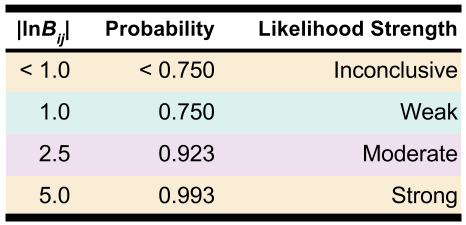
\includegraphics[width=0.4\linewidth]{./figures/evidence-strength.png}
    \caption{Model comparison using likelihood strength}
  \end{table}
  
  posterior probabilities calculated from $\lvert lnB_{ij} \rvert$
  
  Summarize:
  
  Given a mean-squared error and its standard deviation from using CV with any alg, get MLE

  compare two models : $\text{MLE}_i$ to $\text{MLE}_j$
  
  posterior odds is probability of model $i$ being correct
\end{frame}
